\section{Jump Point Search}
Jump Point Search (JPS) is the combination of A* search with 
simple pruning rules that, taken together and applied recursively, 
can identify and eliminate many 
path symmetries from an undirected and 8-connected grid map. %from a given undirected grid map. 
There are two sets of rules: pruning rules and jumping rules. 
\\ \newline
\textbf{Pruning Rules:}
Given a node $x$, reached via a parent node $p$,
we prune from the neighbours of $x$ any node $n$ for which one 
of the following rules applies:
\begin{enumerate}
\item 
  there exists a path $\pi' = \langle p,y,n \rangle$ or simply $\pi' = \langle p, n \rangle$
  that is strictly shorter than the path $\pi = \langle p,x,n \rangle$; 
\item 
  there exists a path $\pi' = \langle p,y,n \rangle$ 
  with the same length as $\pi = \langle p,x,n \rangle$ but $\pi'$ has a 
  diagonal move earlier than $\pi$.  
\end{enumerate}

\begin{figure}[tb]
       \begin{center}
		   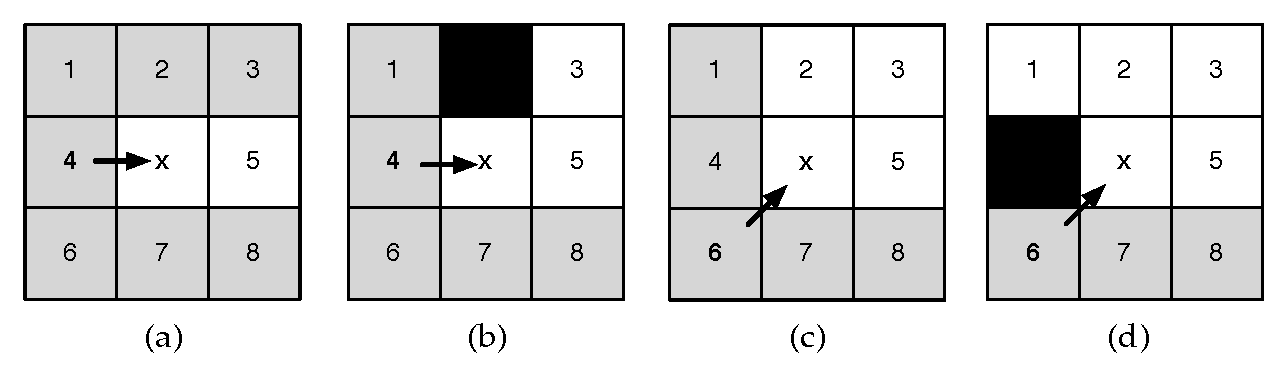
\includegraphics[width=\columnwidth]
			{diagrams/pruningrules.pdf}
       \end{center}
	\vspace{-3pt}
       \caption{\small 
When the move from $p$ to $x$ is straight (as in (a)) only one natural neighbour remains.
When the move from $p$ to $x$ is diagonal (as in (c)), three natural neighbours remain. 
When obstacles are adjacent to $x$  some neighbours become forced; we illustrate this
in for straight moves (q.v. (b)) and for diagonal moves (q.v. (d)).
}
       \label{fig:pruning}
\end{figure}

We illustrate these rules in Figure~\ref{fig:pruning}(a) and ~\ref{fig:pruning}(c).
Observe that to test each rule we need to look only at
the neighbours of the current node $x$. 
Pruned neighbours are marked in grey. Remaining neighbours, marked
white, are called the \emph{natural} successors of node $x$.  
In Figure~\ref{fig:pruning}(b) and ~\ref{fig:pruning}(d) we show
that obstacles can modify the list of successors for $x$:
when the alternative path $\pi' = \langle p, y, n \rangle$ is
not valid, but $\pi = \langle p, x, n \rangle$ is, we will refer to $n$ as
a \emph{forced} successor of $x$.
\\ \newline
\textbf{Jumping Rules:}
JPS applies to each forced and natural neighbour of the current node $x$ a simple recursive
``jumping'' procedure; the objective is to replace each neighbour $n$ with an 
alternative successor $n'$ that is further away. Precise details are given
in~\cite{harabor11b}; we summarise the idea here using a short example:

\begin{example}
In Figure~\ref{fig:pruning}(a) pruning reduces the number
of successors of $x$ to a single node $n = 5$.
JPS exploits this property to immediately and recursively
explore $n$.
If the recursion stops due to an obstacle that blocks further progress
(which is frequently the case), all nodes on the failed path, including $n$, are ignored
and nothing is generated.
Otherwise the recursion leads to a node $n'$ which has a forced
neighbour (or which is the goal). JPS generates $n'$ as a successor of $x$; 
effectively allowing the search to ``jump'' from $x$ directly to $n'$ -- without adding
to the open list any intermediate nodes from along the way.
In Figure~\ref{fig:pruning}(c) node $x$ has three natural neighbours: two straight and one diagonal.
We recurse over the diagonal neighbour only if both straight neighbours produce
failed paths. This ensures we do not miss any potential turning points of the optimal path.
\end{example}

%\begin{figure}[tb]
%       \begin{center}
%		   \includegraphics[width=0.95\columnwidth]
%			{diagrams/jumping.png}
%       \end{center}
%	\vspace{-3pt}
%       \caption{(a) A straight jump from $x$ to $y$; the recursion stops due to node $z$ which is forced.
%(b) A diagonal jump from $x$ to $y$; the recursion stops due to a non-failed straight jump. Continuing 
%would mean missing a potential turn due to $z$.}
%       \label{fig:jumping}
%\end{figure}
%
%In Figure~\ref{fig:jumping}(a) we illustrate a straight jump and in \ref{fig:jumping}(b) a diagonal jump. 
By jumping, JPS is able to move quickly over the map 
without inserting nodes in the A* open list.
This is doubly beneficial as (i) it reduces the number of operations 
and (ii) it reduces the number of nodes in the list, 
making each list operation cheaper.  
Notice that JPS prunes nodes entirely online; the algorithm involves no preprocessing and has no memory overhead.  

